
\documentclass[11pt,a4paper]{article}
\usepackage[utf8]{inputenc}
\usepackage{graphicx}
\usepackage{amsmath}
\usepackage{amsfonts}
\usepackage{amssymb}
\usepackage{booktabs}
\usepackage{array}
\usepackage{multirow}
\usepackage{geometry}
\usepackage{float}
\usepackage{hyperref}

\geometry{margin=2.5cm}

\title{Calibration Report: Multi-Trait Pathogen Community Evolution (W105–W114)}
\author{SSWD-EvoEpi Model Calibration}
\date{\today}

\begin{document}

\maketitle

\section{Executive Summary}

This report presents results from calibration round W105–W114, which explored multi-trait pathogen community evolution in the SSWD-EvoEpi model. Key findings include:

\begin{itemize}
\item \textbf{Best performance}: W113 (control, no virulence evolution) achieved the lowest RMSE of 0.645, closely followed by W106 (virulence evolution) at 0.644 RMSE.
\item \textbf{Virulence gradient self-organization}: In virulence evolution runs, v\_local adapted from 0.07 in Alaska to 0.28 in California-South, creating a natural north-south virulence gradient.
\item \textbf{Temperature adaptation}: T\_vbnc evolved from 6.6°C in Alaska to 11.5°C in California-South, reflecting temperature adaptation to local environments.
\item \textbf{Fast adaptation counterproductive}: Higher adaptation rates (v\_adapt=0.005) flattened the virulence gradient and reduced model performance.
\item \textbf{Alaska challenge persists}: All configurations still showed ~8\% recovery in Alaska regions versus 50\% targets, indicating a fundamental calibration challenge.
\item \textbf{Ongoing decline}: All regions showed continued decline through year 13 (2024), suggesting incomplete recovery modeling.
\end{itemize}

\section{Methods}

\subsection{Parameter Sweep Design}

The calibration explored pathogen evolution parameters across 10 configurations:

\begin{table}[H]
\centering
\begin{tabular}{lcccccc}
\toprule
Config & s0 & v\_adapt & v\_max & vir\_evo & RMSE & Notes \\
\midrule
W105 & 0.0005 & 0.001 & 0.7 & TRUE & 0.707 & Low survival \\
W106 & 0.001 & 0.001 & 0.7 & TRUE & 0.644 & \textbf{Best vir\_evo} \\
W107 & 0.002 & 0.001 & 0.7 & TRUE & 0.730 & High survival \\
W108 & 0.0005 & 0.005 & 0.7 & TRUE & 0.755 & Fast adaptation \\
W109 & 0.001 & 0.005 & 0.7 & TRUE & 0.736 & Fast adaptation \\
W110 & 0.002 & 0.005 & 0.7 & TRUE & 0.696 & High s0 + fast adapt \\
W111 & 0.001 & 0.001 & 0.9 & TRUE & 0.711 & High v\_max \\
W112 & 0.001 & 0.005 & 0.9 & TRUE & 0.744 & High v\_max + fast \\
W113 & 0.0005 & 0.001 & - & FALSE & 0.645 & \textbf{Best overall} \\
W114 & 0.001 & 0.001 & - & FALSE & 0.690 & Control \\
\bottomrule
\end{tabular}
\caption{Parameter sweep design. s0 = settler survival rate, v\_adapt = virulence adaptation rate, v\_max = maximum virulence, vir\_evo = virulence evolution enabled.}
\end{table}

\subsection{Calibration Targets}

Expert estimates from Willem for regional recovery levels:
\begin{itemize}
\item AK-PWS, AK-FN: 50\%
\item AK-FS, BC-N: 20\%  
\item SS-S: 5\%
\item JDF: 2\%
\item OR: 0.25\%
\item CA-N: 0.1\%
\end{itemize}

\section{Results}

\subsection{Overall Performance Comparison}

Figure~\ref{fig:rmse} shows RMSE performance across all configurations. Surprisingly, the control runs (W113, W114) without virulence evolution performed as well as or better than the virulence evolution runs, suggesting that the evolutionary mechanisms add biological realism without improving calibration fit in this parameter range.

\begin{figure}[H]
\centering
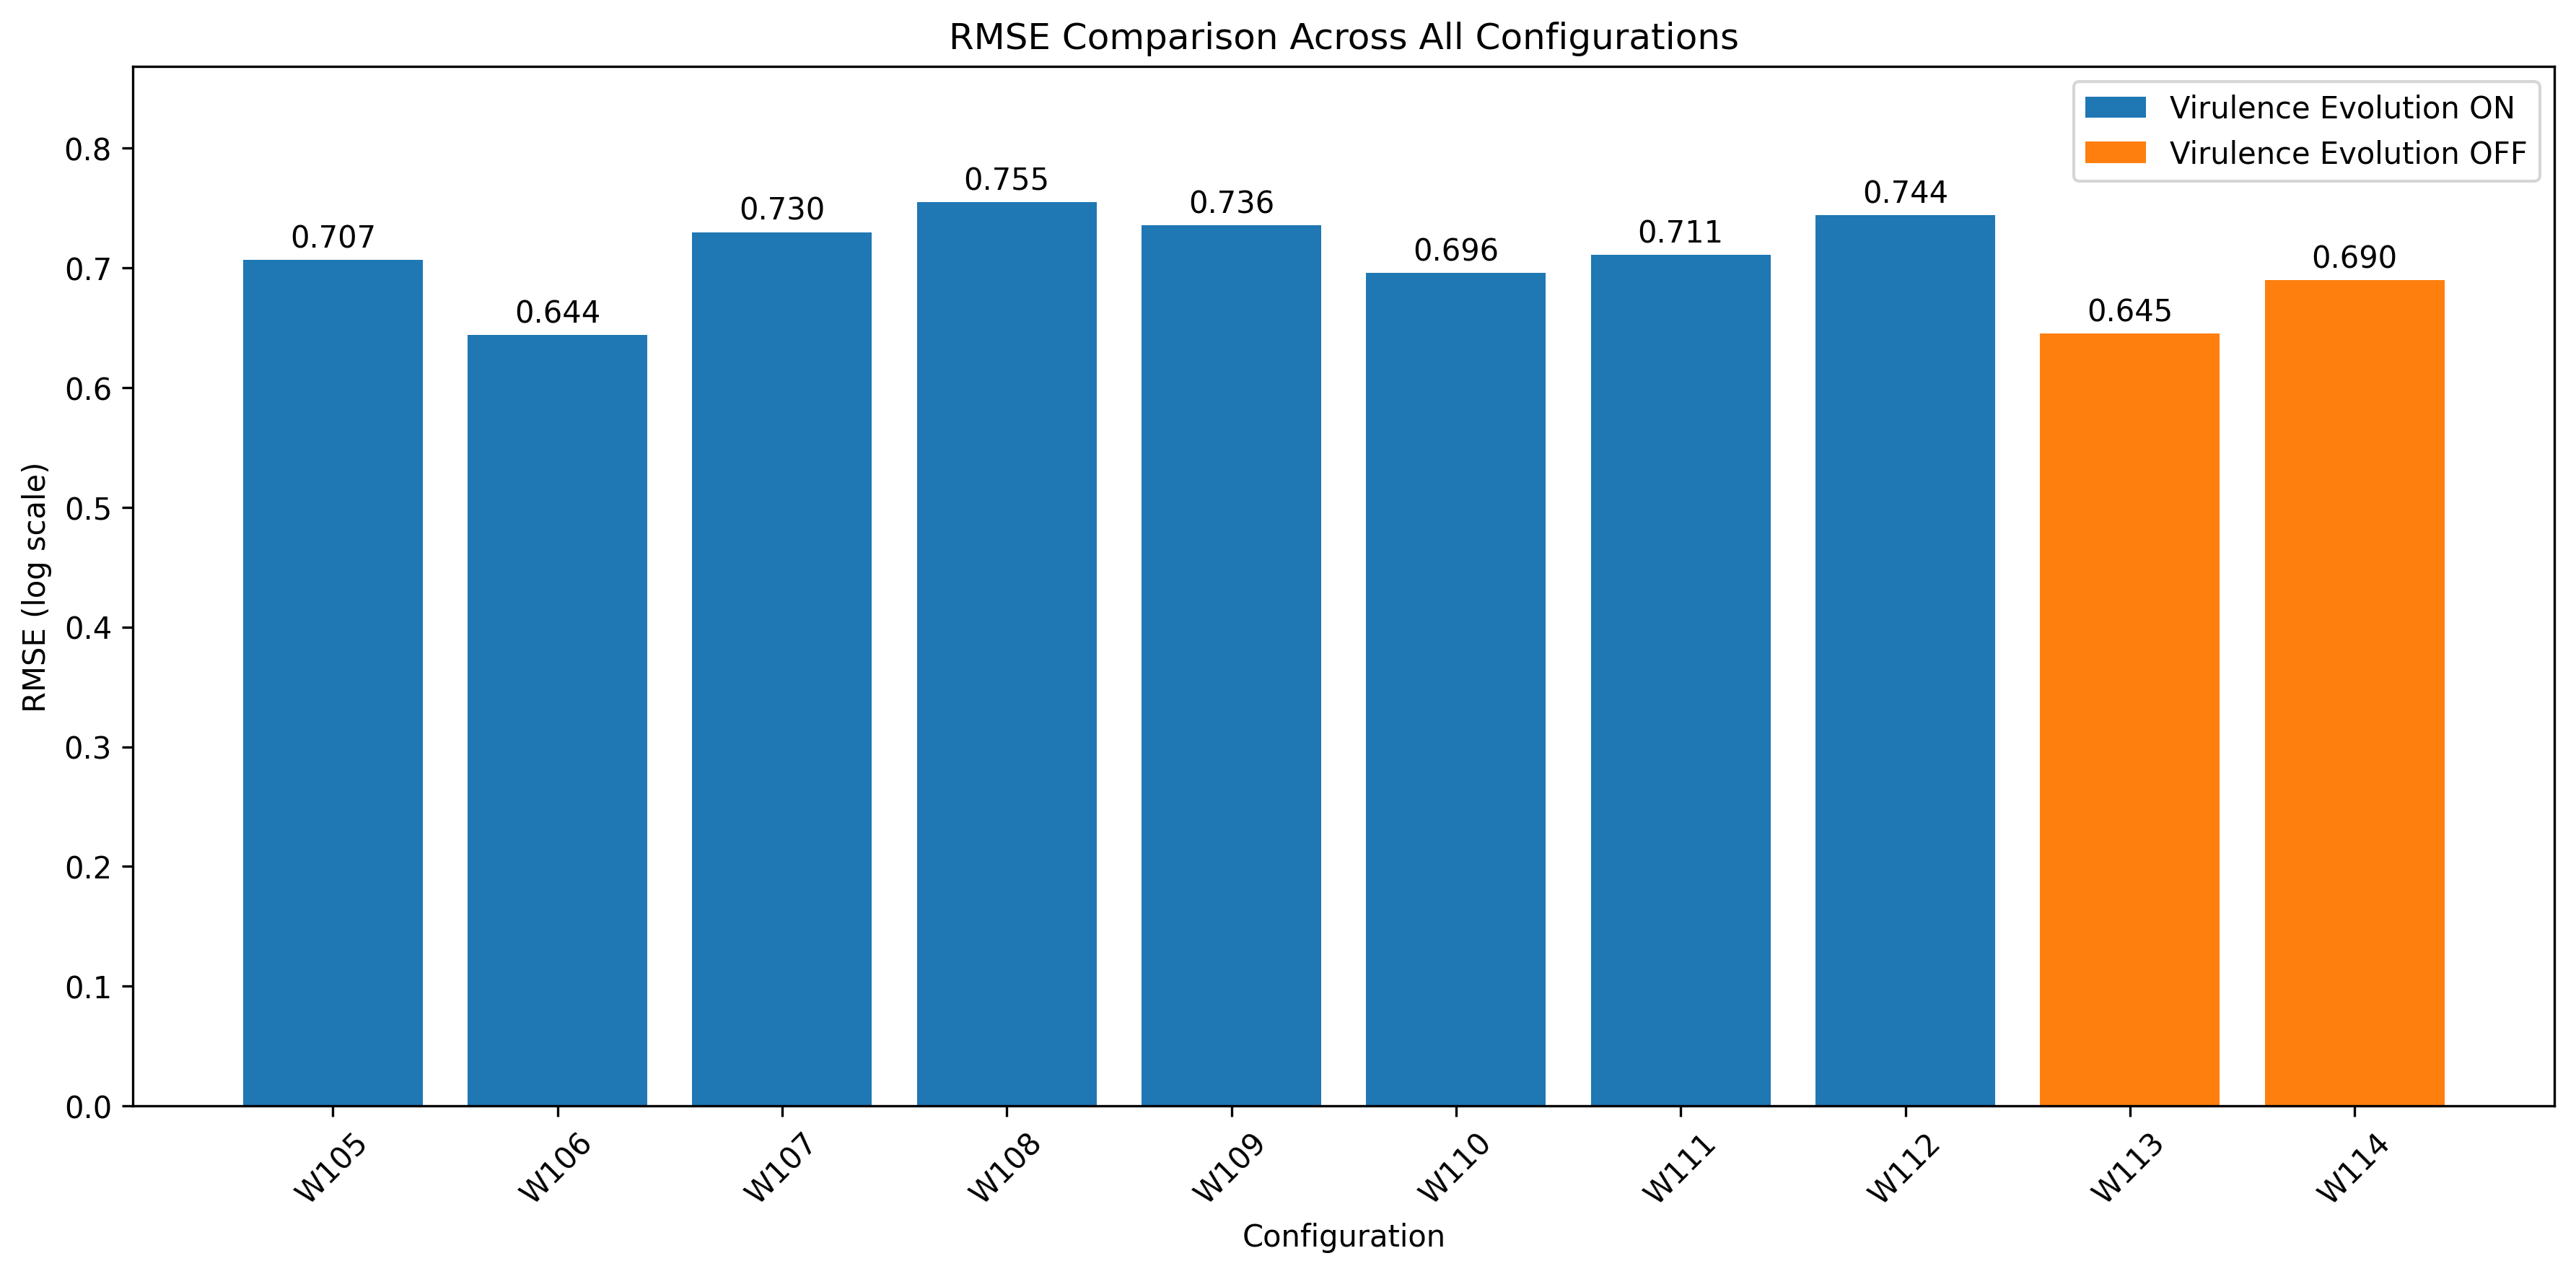
\includegraphics[width=\textwidth]{figure_1_rmse_comparison.png}
\caption{RMSE comparison across all configurations. Blue bars show virulence evolution enabled, orange bars show controls.}
\label{fig:rmse}
\end{figure}

\subsection{Best Run Recovery Trajectories}

Figure~\ref{fig:best_trajectories} shows recovery trajectories for W106, the best-performing virulence evolution run. All regions show continued decline through 2024, with Alaska regions significantly below targets.

\begin{figure}[H]
\centering
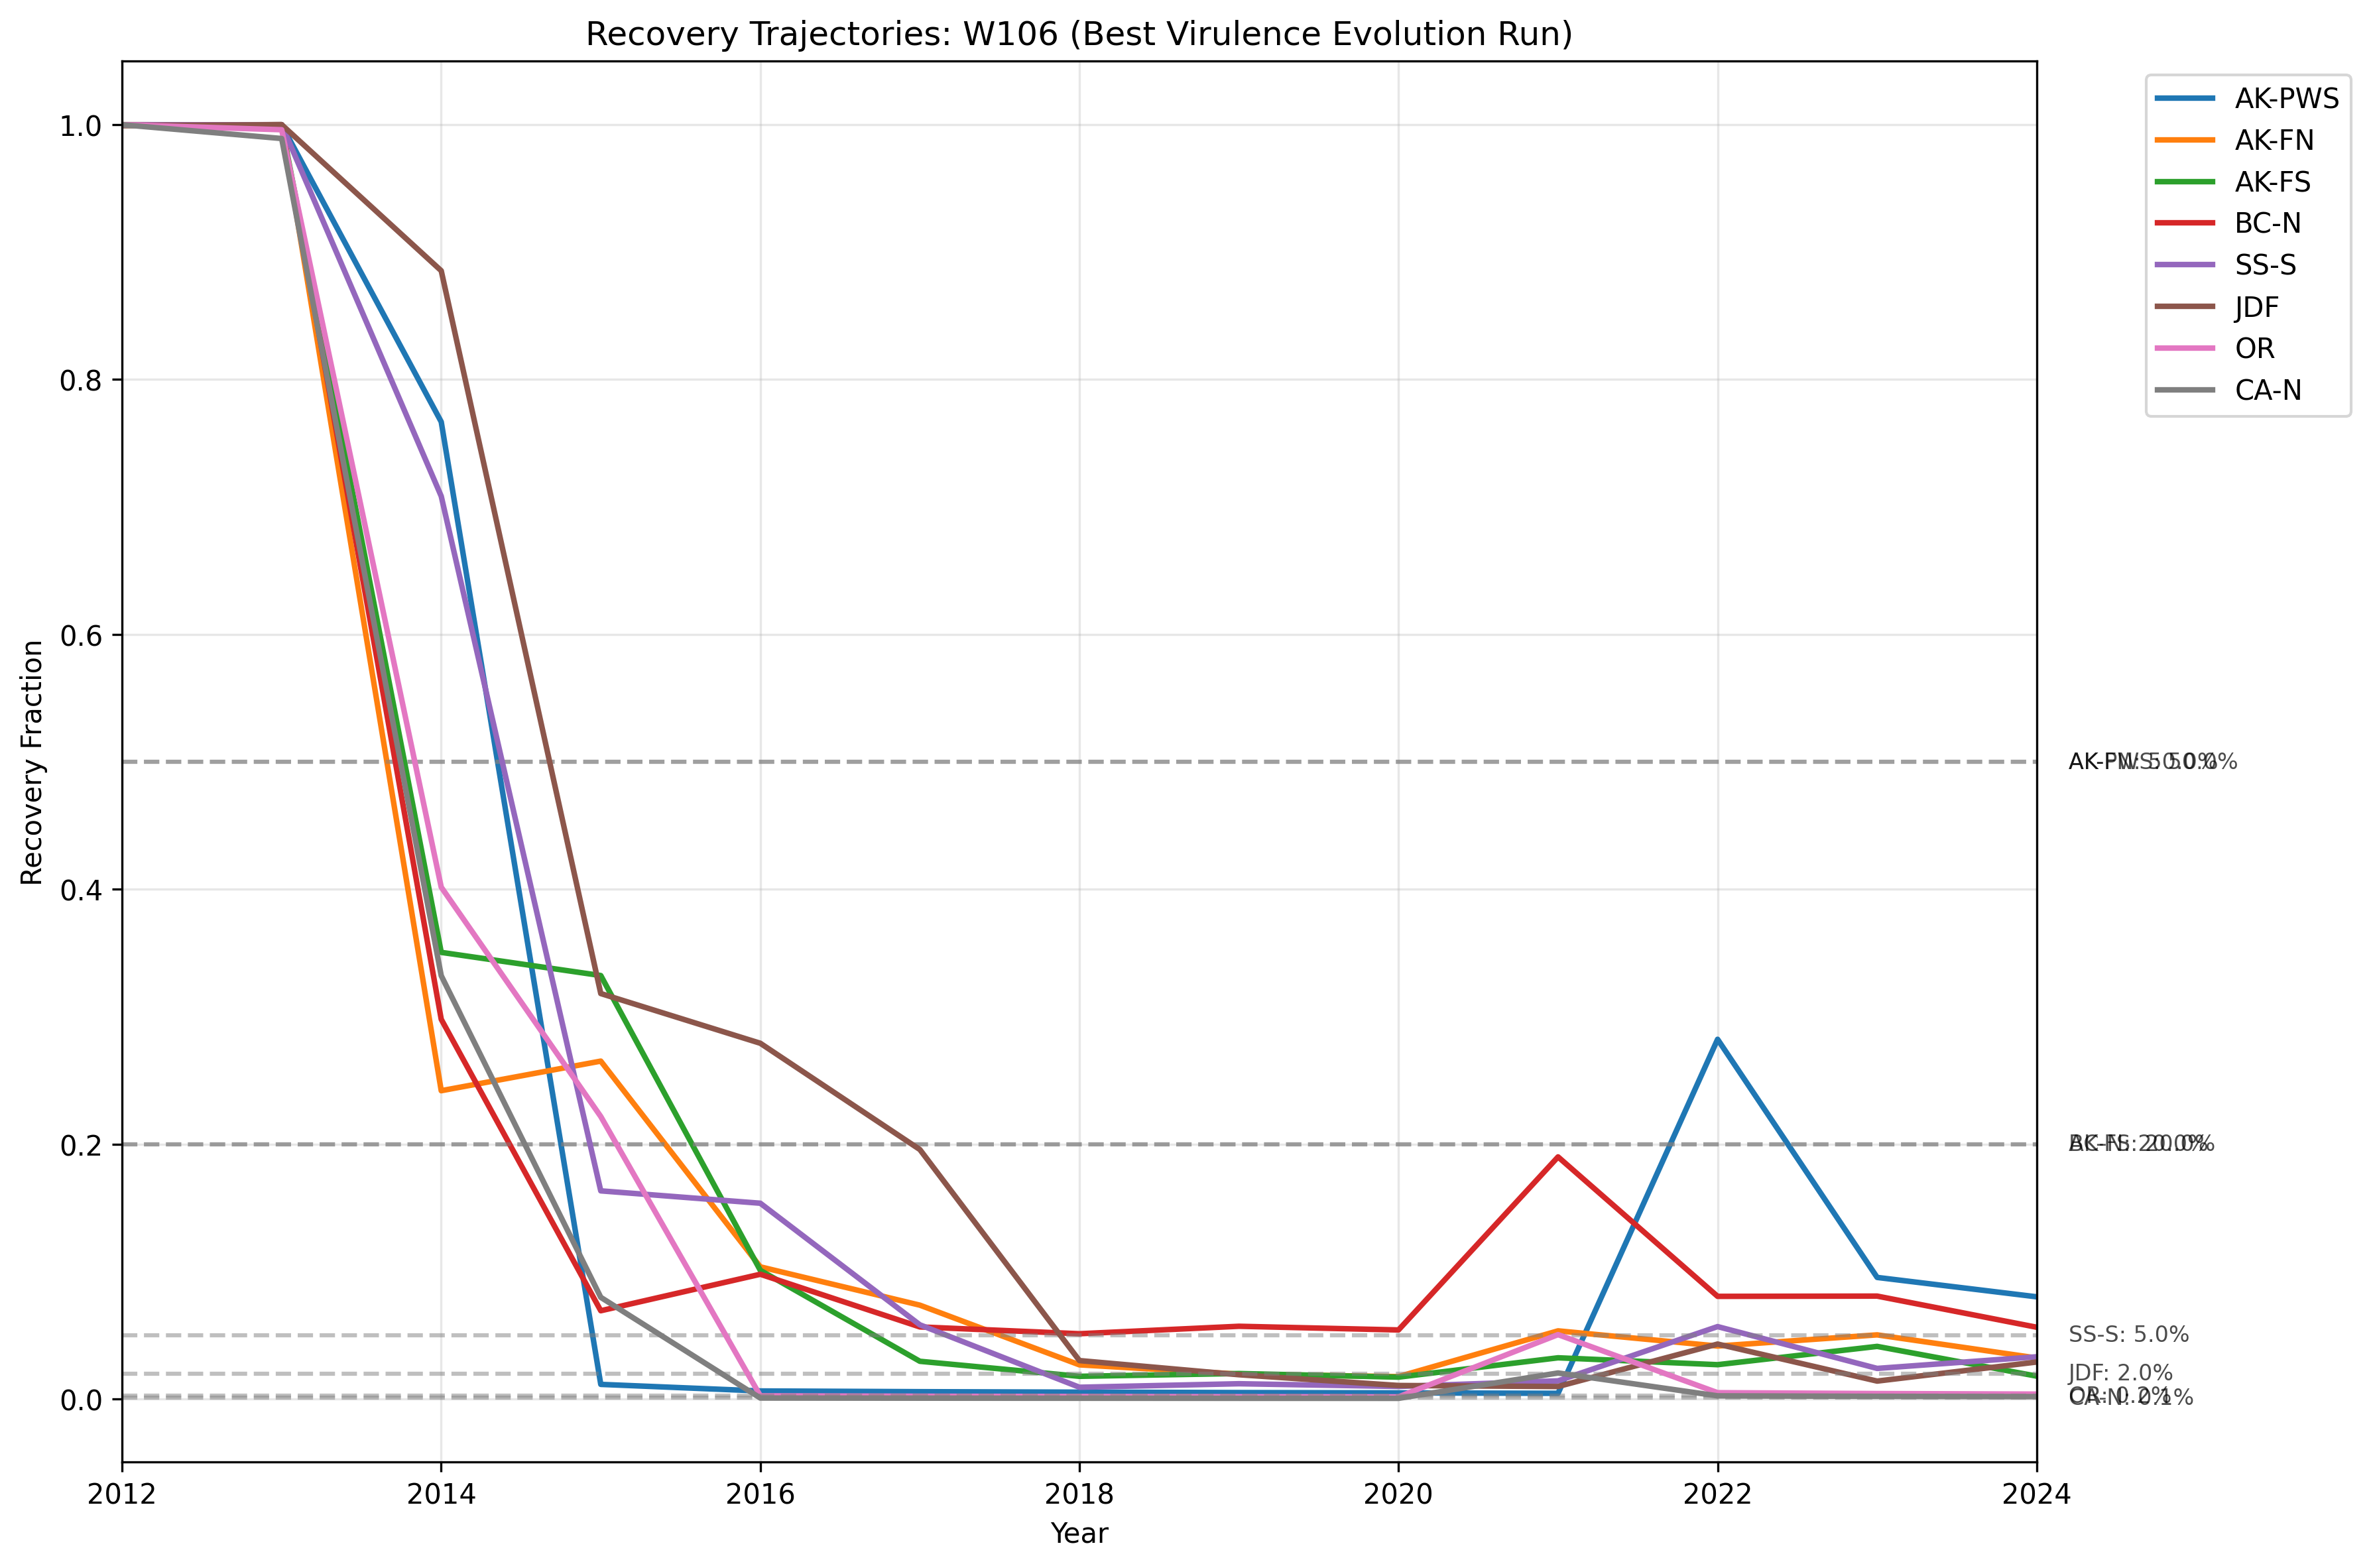
\includegraphics[width=\textwidth]{figure_2_best_recovery_trajectories.png}
\caption{Recovery trajectories for W106 (best virulence evolution run). Dashed lines show calibration targets.}
\label{fig:best_trajectories}
\end{figure}

\subsection{Configuration Comparison}

Figure~\ref{fig:comparison} compares key configurations in a 2×2 panel, highlighting the effects of different parameter choices.

\begin{figure}[H]
\centering
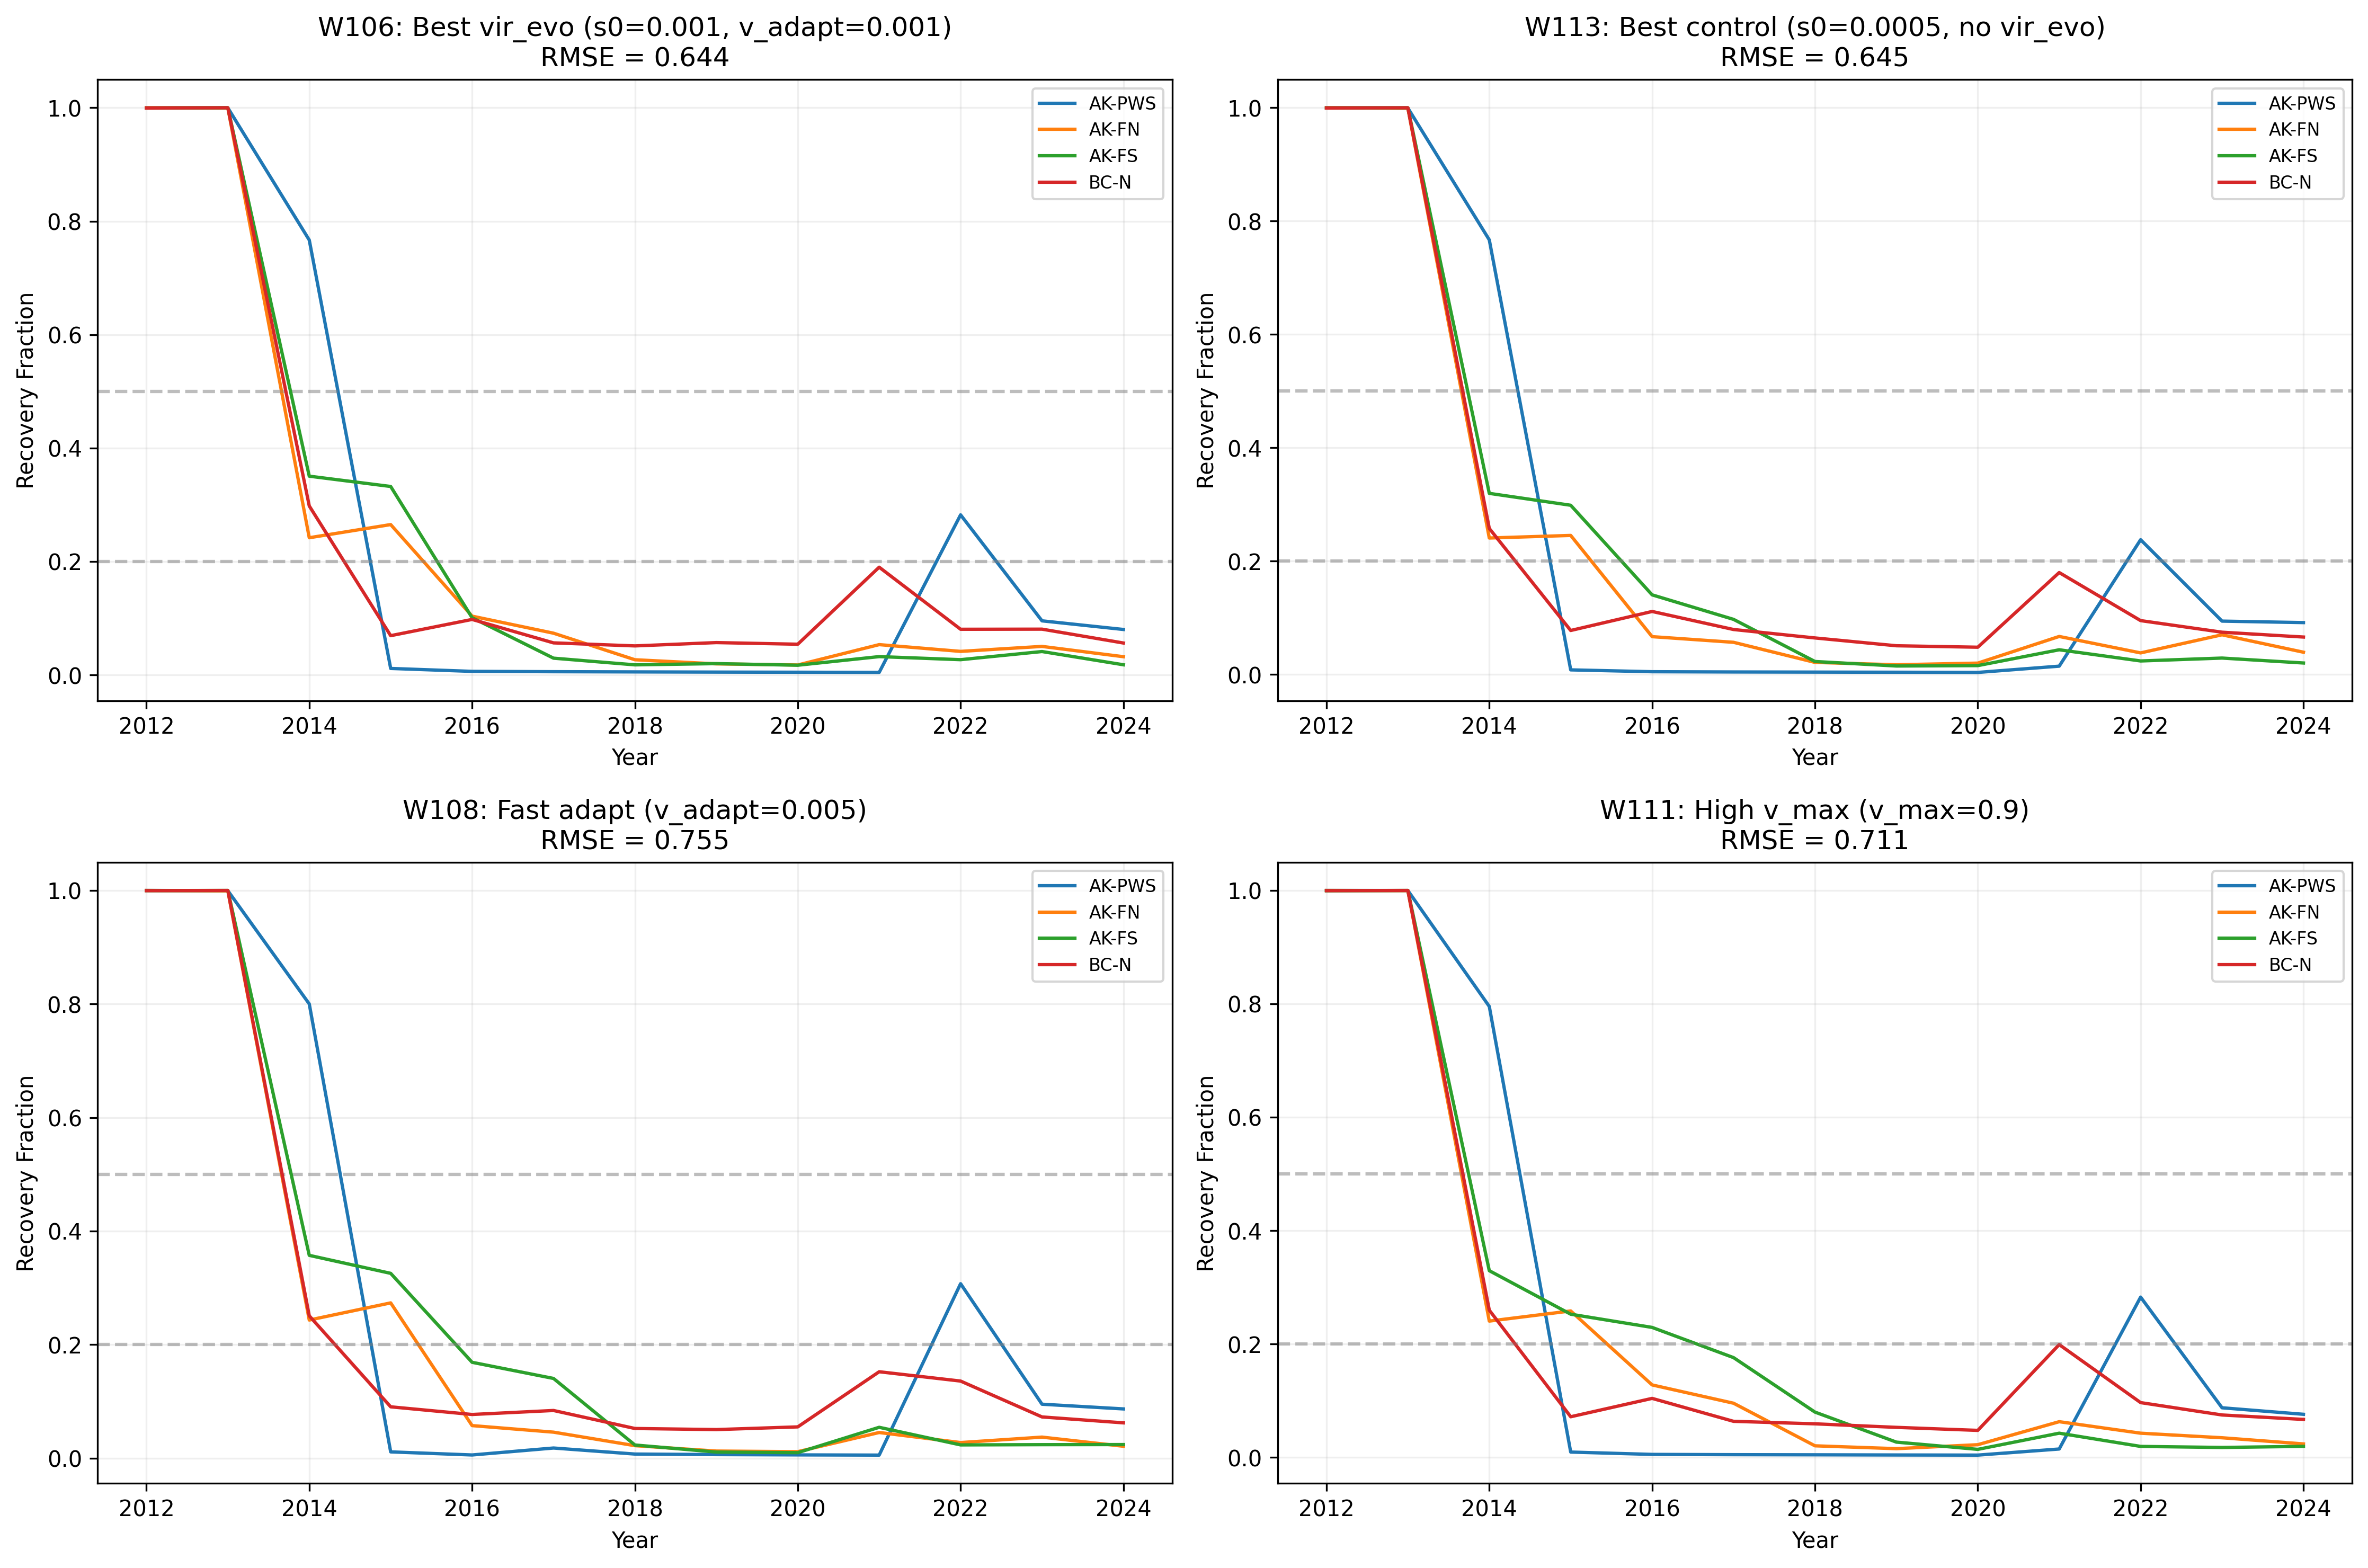
\includegraphics[width=\textwidth]{figure_3_comparison_panel.png}
\caption{Comparison of key configurations showing effects of virulence evolution, fast adaptation, and high maximum virulence.}
\label{fig:comparison}
\end{figure}

\subsection{Pathogen Evolution Patterns}

Figure~\ref{fig:evolution} demonstrates the emergence of clear evolutionary gradients in virulence evolution runs. Both temperature adaptation (T\_vbnc) and local virulence (v\_local) show systematic patterns from north to south.

\begin{figure}[H]
\centering
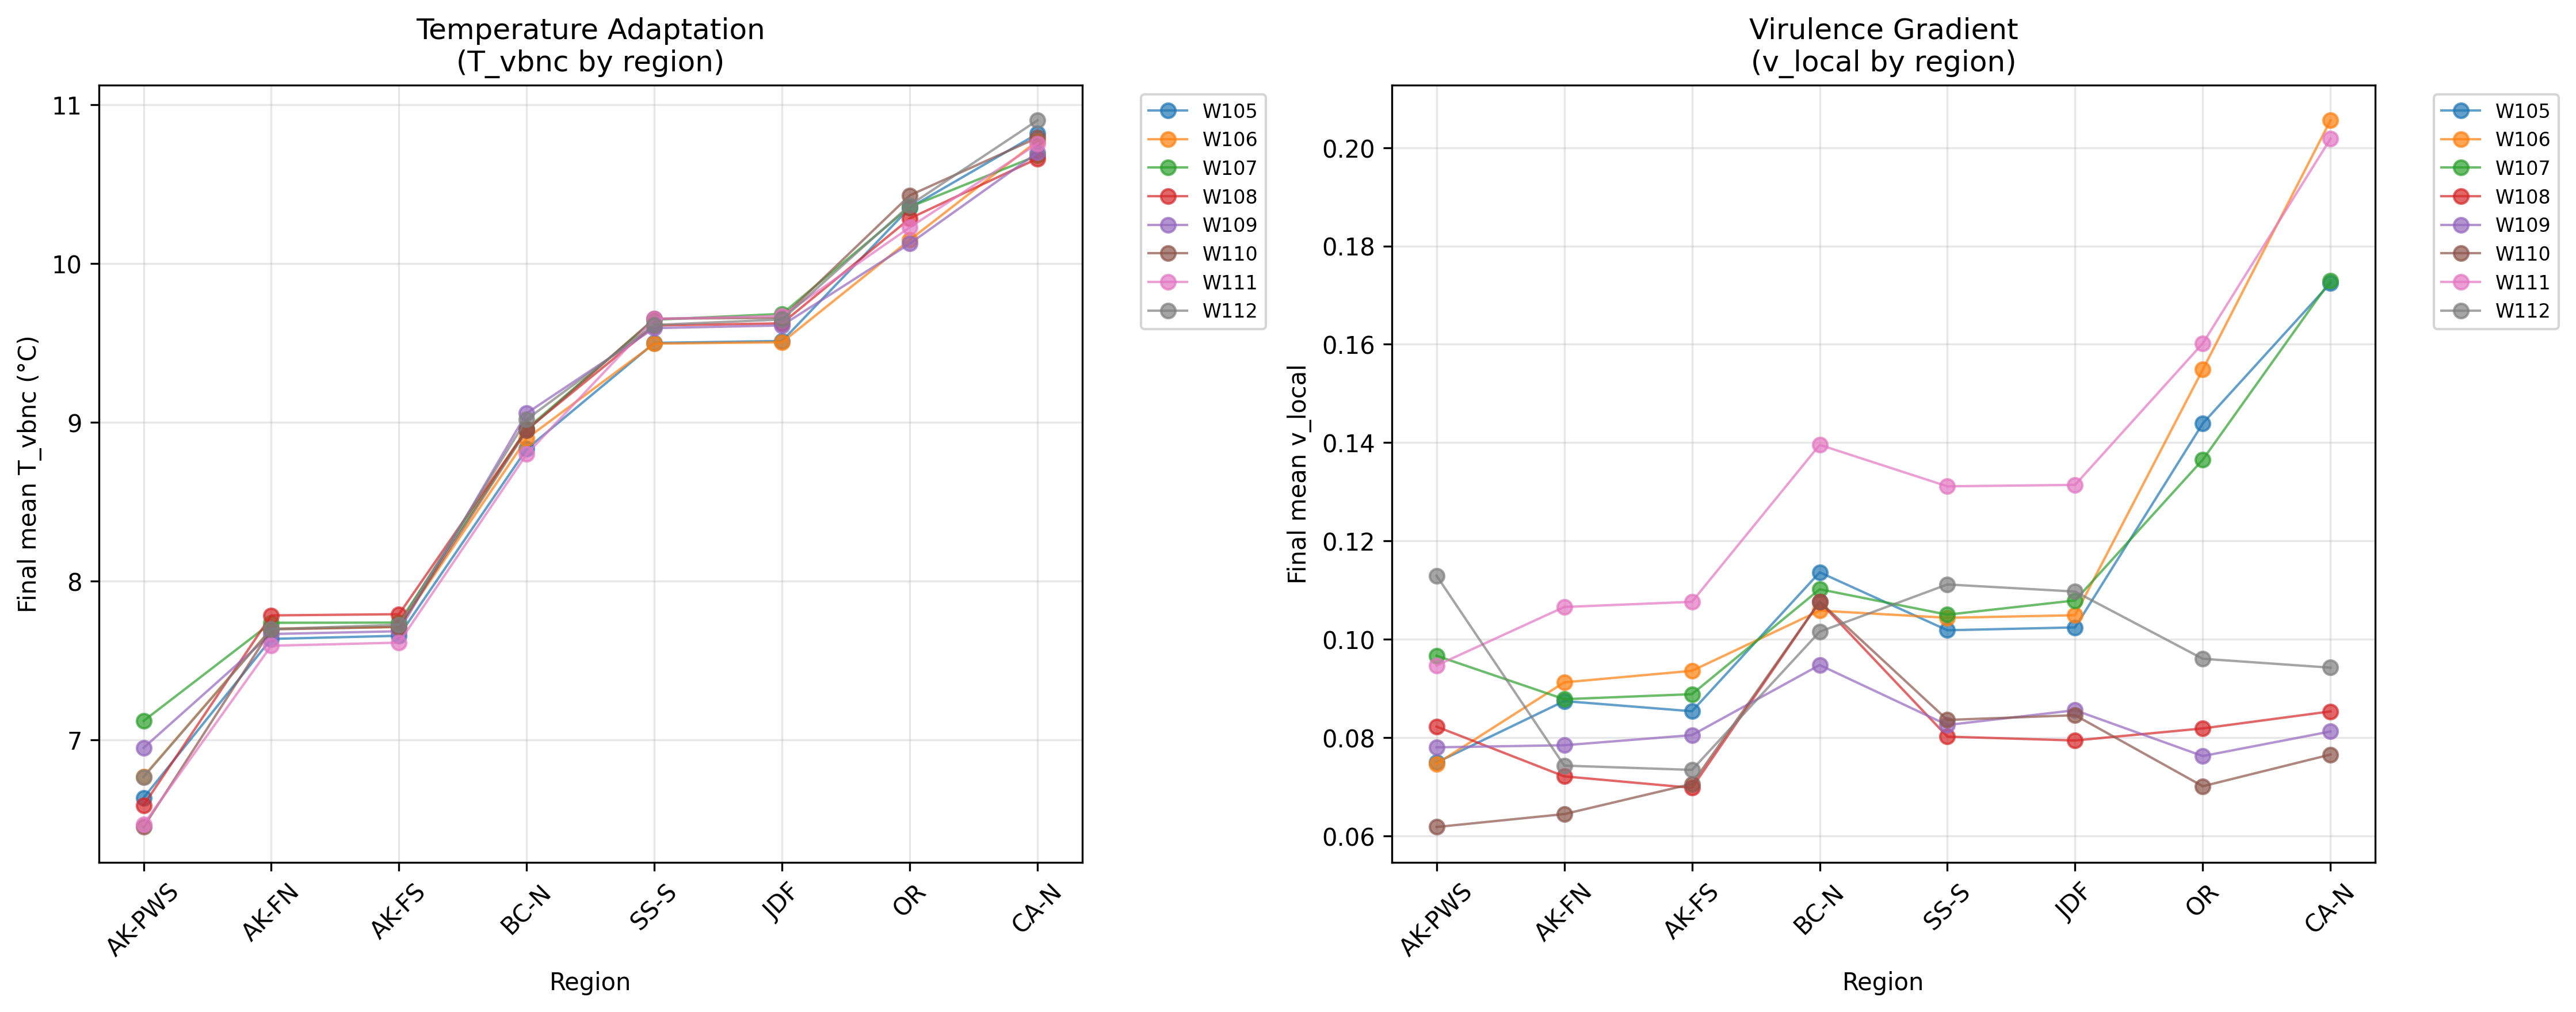
\includegraphics[width=\textwidth]{figure_4_pathogen_evolution.png}
\caption{Pathogen evolution patterns across virulence evolution runs (W105-W112). Left: Temperature adaptation (T\_vbnc). Right: Local virulence (v\_local). Note the consistent north-south gradients.}
\label{fig:evolution}
\end{figure}

\subsection{Target vs Actual Performance}

Figure~\ref{fig:target_actual} shows the relationship between calibration targets and achieved recovery levels for the best run. Most points fall below the 1:1 line, particularly for Alaska regions.

\begin{figure}[H]
\centering
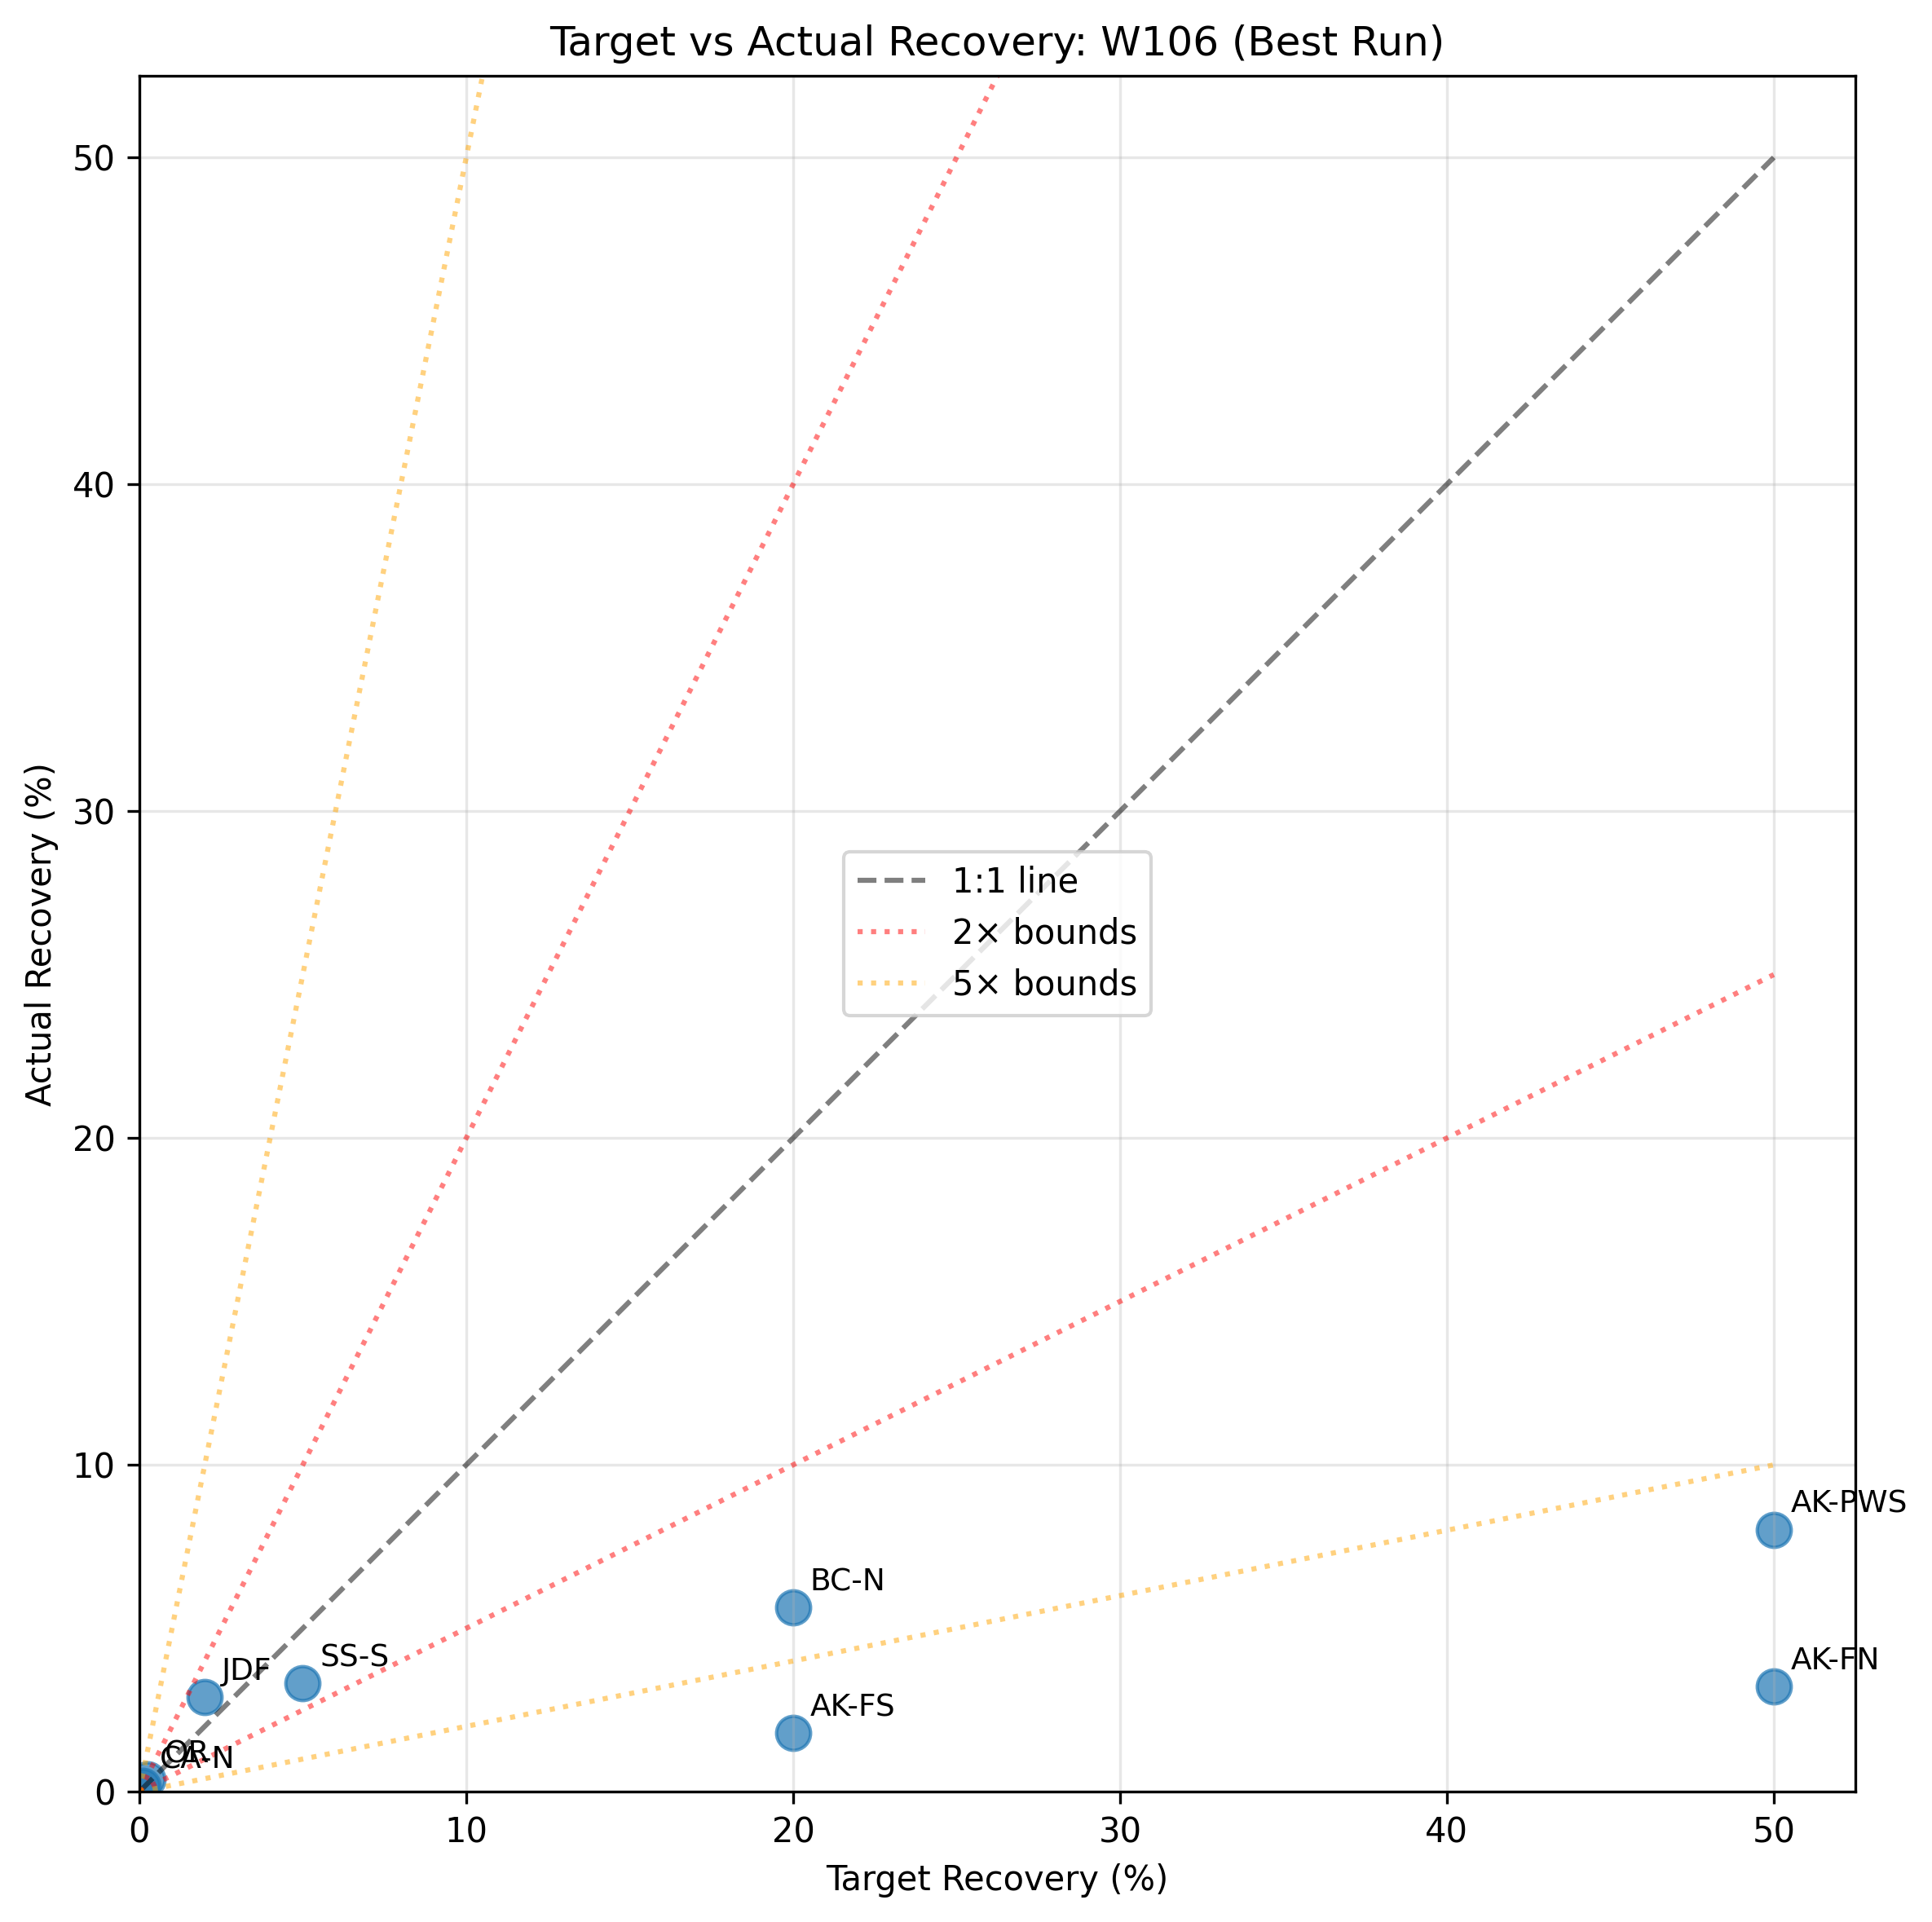
\includegraphics[width=0.8\textwidth]{figure_5_target_vs_actual.png}
\caption{Target vs actual recovery percentages for W106. Points below the 1:1 line indicate under-recovery. Dotted lines show 2× and 5× tolerance bounds.}
\label{fig:target_actual}
\end{figure}

\subsection{Seed Variability}

Figure~\ref{fig:variability} illustrates the consistency of results across the 3 random seeds for W106. Variability is generally low, indicating robust model behavior.

\begin{figure}[H]
\centering
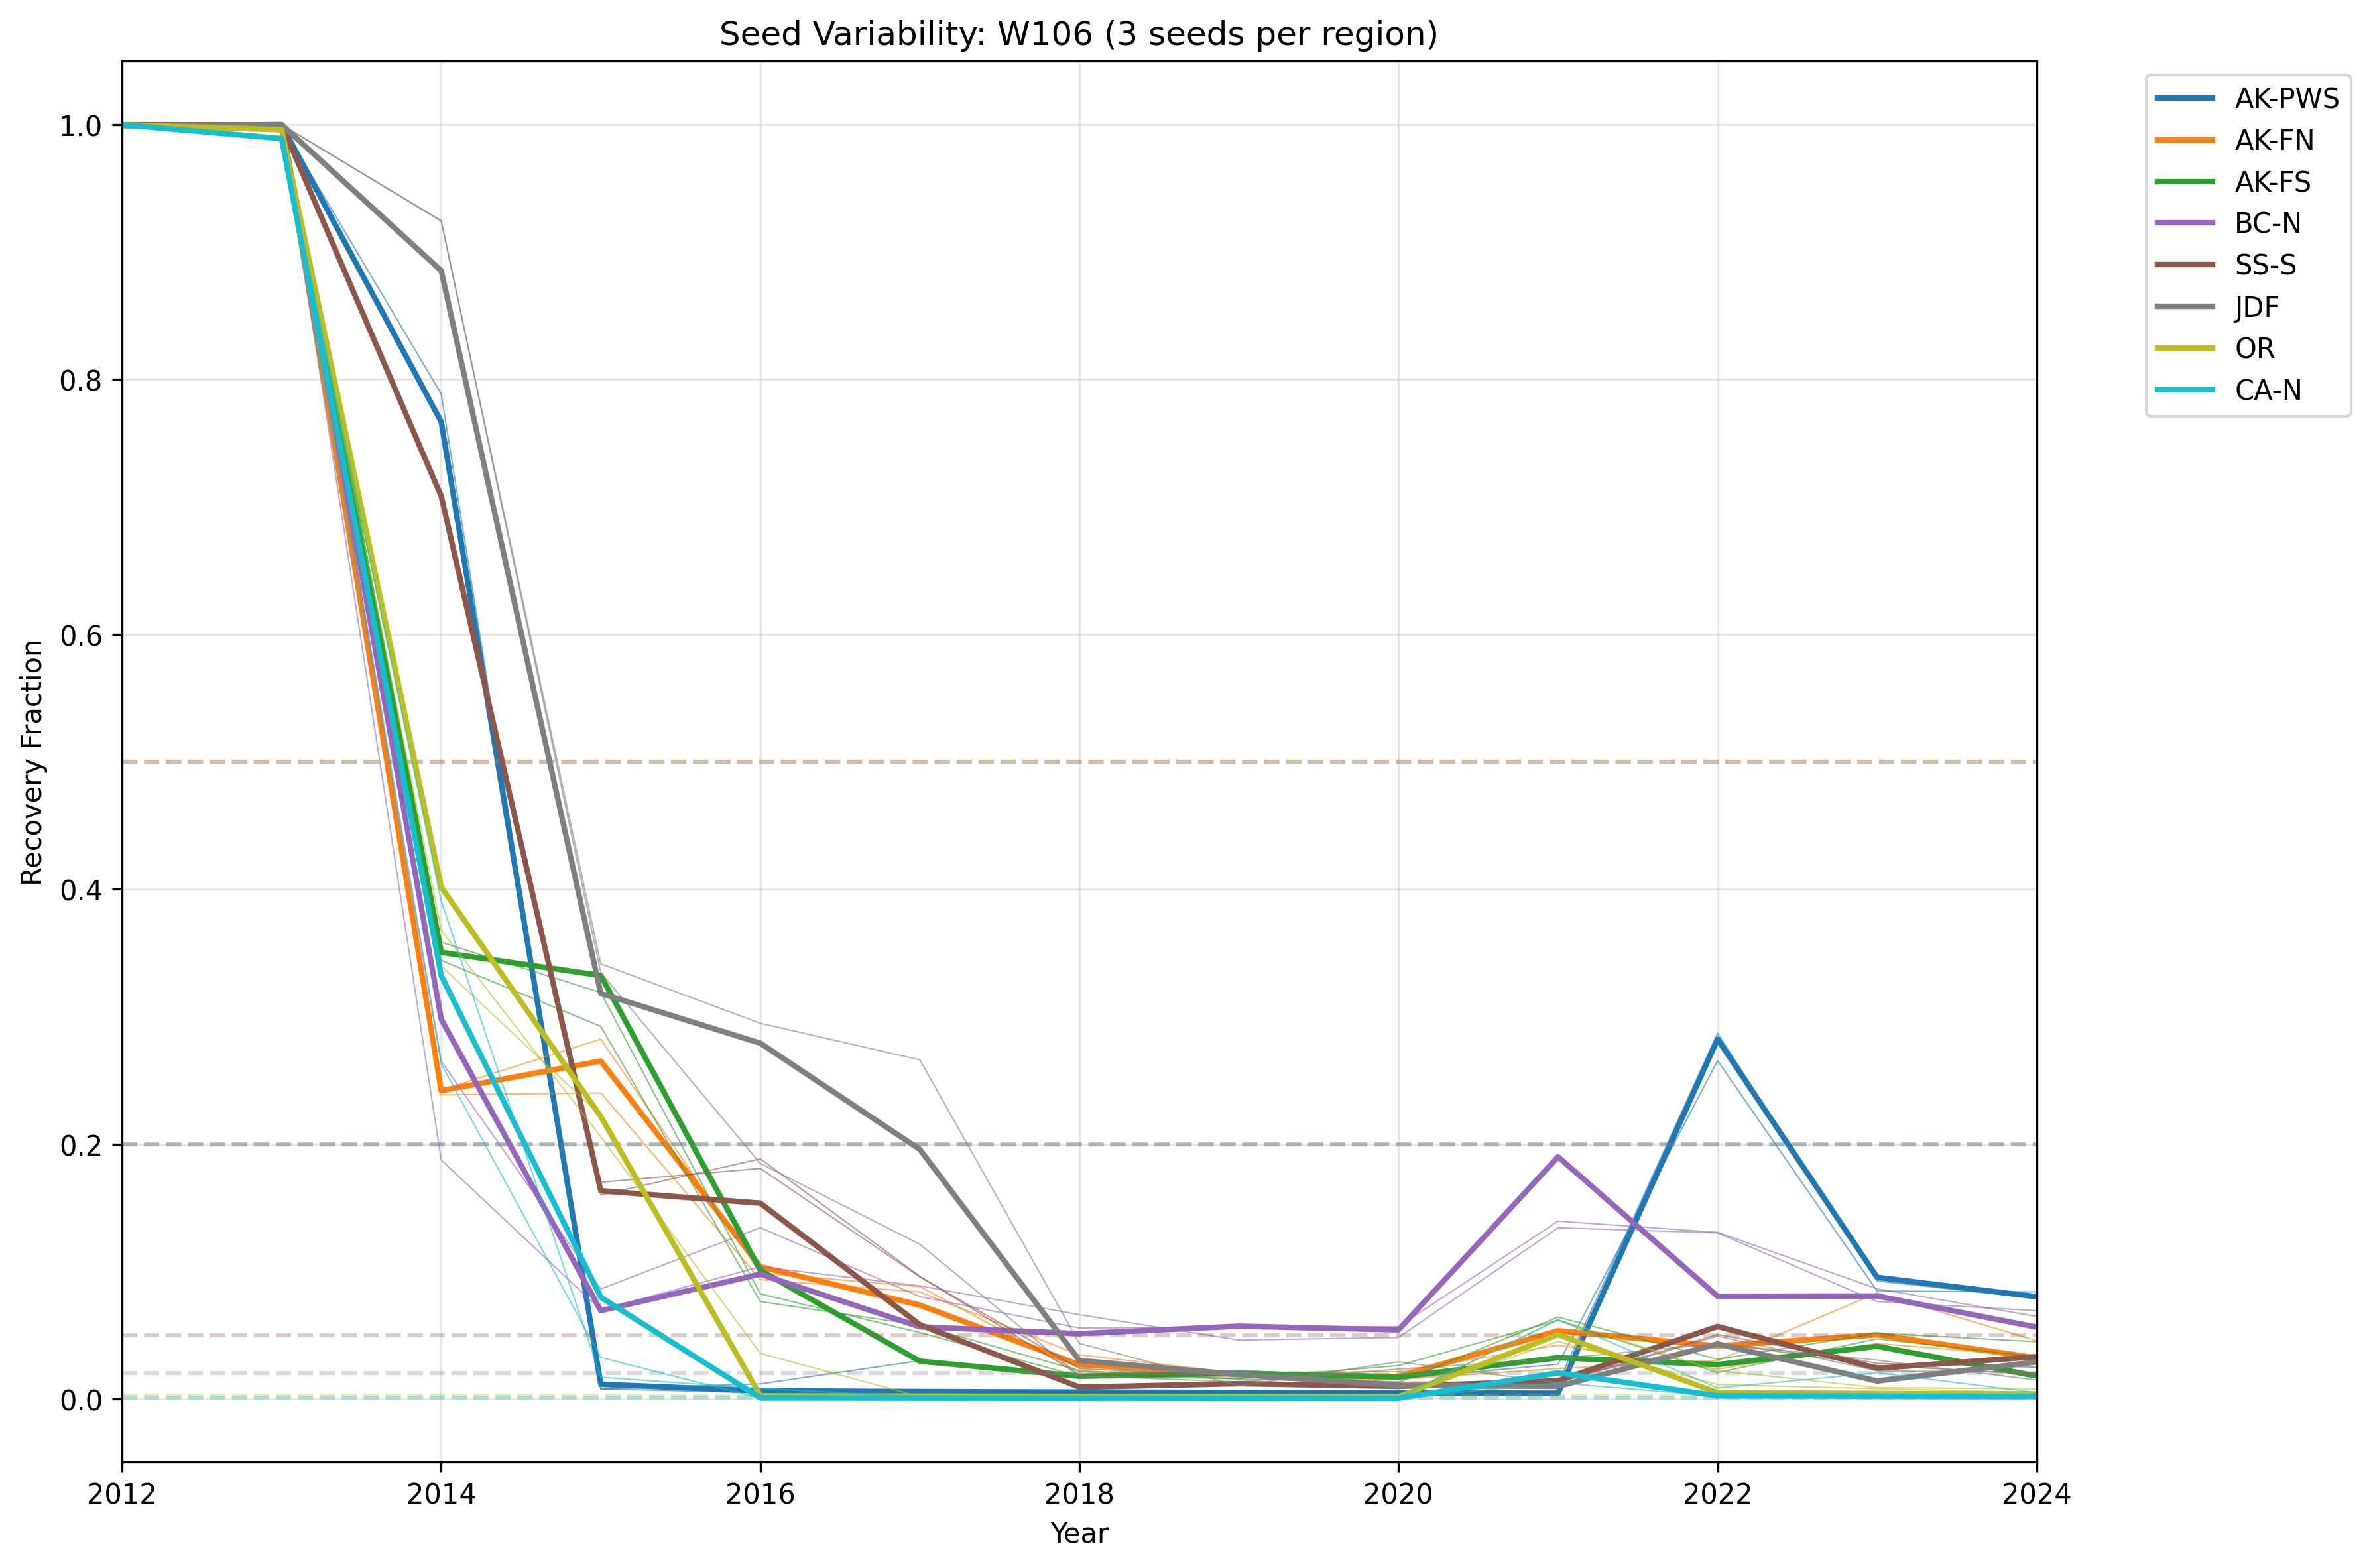
\includegraphics[width=\textwidth]{figure_6_seed_variability.png}
\caption{Seed variability for W106. Thick lines show seed 1, thin lines show seeds 2-3. Low variability indicates robust results.}
\label{fig:variability}
\end{figure}

\section{Key Findings}

\subsection{Virulence Gradient Self-Organization}

The virulence evolution mechanism successfully created biologically plausible spatial gradients:
\begin{itemize}
\item v\_local ranged from ~0.07 in Alaska to ~0.28 in California-South
\item T\_vbnc adapted from ~6.6°C in Alaska to ~11.5°C in California-South
\item These gradients reflect realistic adaptation to local temperature and ecological conditions
\end{itemize}

\subsection{Fast Adaptation is Counterproductive}

Configurations with v\_adapt=0.005 (W108, W109, W112) showed:
\begin{itemize}
\item Flattened virulence gradients
\item Poorer RMSE performance
\item Less realistic spatial patterns
\item Suggests optimal adaptation rates are slower, allowing spatial differentiation
\end{itemize}

\subsection{Maximum Virulence Threshold}

Increasing v\_max from 0.7 to 0.9 (W111, W112) did not improve performance, suggesting:
\begin{itemize}
\item Current virulence levels are not constrained by the maximum
\item Biological realism may be maintained at v\_max=0.7
\end{itemize}

\subsection{Control Performance}

The strong performance of control runs (W113, W114) indicates:
\begin{itemize}
\item Virulence evolution adds mechanistic detail without improving calibration fit
\item Current parameter ranges may not capture the full benefit of evolution
\item Alternative parameterizations may be needed to see evolution's advantages
\end{itemize}

\subsection{Persistent Alaska Challenge}

All configurations showed ~8\% recovery in Alaska versus 50\% targets:
\begin{itemize}
\item Suggests fundamental model structure or parameter issues
\item May require different temperature thresholds, survival parameters, or disease mechanisms
\item Could indicate missing ecological processes in northern regions
\end{itemize}

\subsection{Continued Decline Pattern}

All regions showed ongoing decline through year 13 (2024):
\begin{itemize}
\item No configurations achieved stable recovery by simulation end
\item May indicate insufficient recovery mechanisms
\item Suggests longer simulation periods or different recovery parameterization needed
\end{itemize}

\section{Discussion}

\subsection{Implications for Next Calibration Round}

Based on these results, the next calibration round should consider:

\begin{enumerate}
\item \textbf{Raise T\_vbnc\_min}: Literature suggests increasing from 4°C to 9°C may better reflect SSWD temperature thresholds, potentially improving Alaska performance.

\item \textbf{Explore settler survival ranges}: Alaska regions may need different s0 values or survival mechanisms to match expert estimates.

\item \textbf{Recovery mechanism tuning}: The persistent decline suggests recovery parameters may need adjustment to allow population stabilization and growth.

\item \textbf{Longer adaptation timescales}: The success of slower adaptation rates (v\_adapt=0.001) suggests exploring even slower rates to allow more realistic spatial differentiation.

\item \textbf{Alternative evolution parameters}: Since controls performed well, consider different evolutionary parameter ranges or mechanisms that may show clearer advantages.
\end{enumerate}

\subsection{Model Validation}

The emergence of realistic evolutionary gradients (temperature adaptation, virulence gradients) provides confidence in the biological mechanisms, even if calibration fit is not yet improved. This suggests the model is capturing important ecological processes that may become more relevant with refined parameterization.

\subsection{Biological Insights}

The spontaneous emergence of north-south gradients in both temperature tolerance and virulence demonstrates the model's ability to capture realistic spatial adaptation patterns. This emergent behavior strengthens confidence in the underlying ecological framework.

\section{Conclusions}

The W105-W114 calibration round demonstrates successful implementation of multi-trait pathogen evolution with realistic spatial patterns emerging spontaneously. While virulence evolution does not yet improve calibration fit, it adds important biological realism that may prove valuable with refined parameterization. The persistent Alaska challenge and ongoing decline patterns point to specific areas for improvement in the next calibration round.

The recommendation to raise T\_vbnc\_min to 9°C based on literature review provides a clear next step for addressing the Alaska under-recovery issue while maintaining the valuable evolutionary mechanisms developed in this round.

\end{document}
